\documentclass[10pt,a4paper]{article}
\usepackage[utf8]{inputenc}

% \usepackage{ngerman}  % german documents
\usepackage{graphicx}  % import graphics einbinden
\usepackage{listings}  % support source code listing
\usepackage{amsmath}  % math stuff
\usepackage{amssymb} % 
\usepackage{a4wide} % wide pages
\usepackage{fancyhdr} % nice headers
\usepackage{tikz} %graphs
\usetikzlibrary{arrows}
\lstset{basicstyle=\footnotesize,language=Python,numbers=left, numberstyle=\tiny, stepnumber=5,firstnumber=0, numbersep=5pt} % set up listings
\pagestyle{fancy}             % header
\setlength{\parindent}{0pt}   % no indentation

\usepackage[pdfpagemode=None, colorlinks=true,  % url coloring
           linkcolor=blue, urlcolor=blue, citecolor=blue, plainpages=false, 
           pdfpagelabels,unicode]{hyperref}
           
% change enums style: first level (a), (b), (c)           
\renewcommand{\labelenumi}{(\alph{enumi})}
\renewcommand{\labelenumii}{(\arabic{enumii})}

%lecture name
\newcommand{\lecture}{
	Bioinformatics III
}           

%assignment iteration
\newcommand{\assignment}{
	Fifth Assignment
}

%set up names, matricle number, and email
\newcommand{\authors}{
  \begin{tabular}{rl}
    \href{mailto:s9alfloh@stud.uni-saarland.de}{Alexander Flohr} & (2549738)\\
    \href{mailto:s9ankupi@stud.uni-saarland.de}{Andrea Kupitz} & (2550260)
  \end{tabular}
}

% use to start a new exercise
\newcommand{\exercise}[1]
{
  \stepcounter{subsection}
  \subsection*{Exercise \thesubsection: #1}

}

\begin{document}
\title{\Large \lecture \\ \textbf{\normalsize \assignment}}
\author{\authors}

\setlength \headheight{25pt}
\fancyhead[R]{\begin{tabular}{r}\lecture \\ \assignment \end{tabular}}
\fancyhead[L]{\authors}


\setcounter{section}{5} % modify for later sheets, i.e. 2, 3, ...
%\section{Introduction to Python and some Network Properties} % optional, note that section invocation sets the section counter + 1, so adapt the setcounter command
\maketitle

\exercise{Cliques and Network Evolution}
\begin{enumerate}
\item Listing \ref{ex1-1} shows source code.
\lstinputlisting[label=ex1-1,caption={Listing of source code}] {CliqueNetwork.py}

\item Listing \ref{ex1-1} shows source code.

\item Listing \ref{ex1-1} shows source code.

\item The number of cliques stays approximately the same independent of the time step because approximately the same amount of edges are added which are removed as shown in figure \ref{fig-1}, table \ref{tab1} and table \ref{tab2}. The amount of cliques of size 3 increases rather than the one of larger cliques because a less edges added may result in a small clique.
\begin{figure}
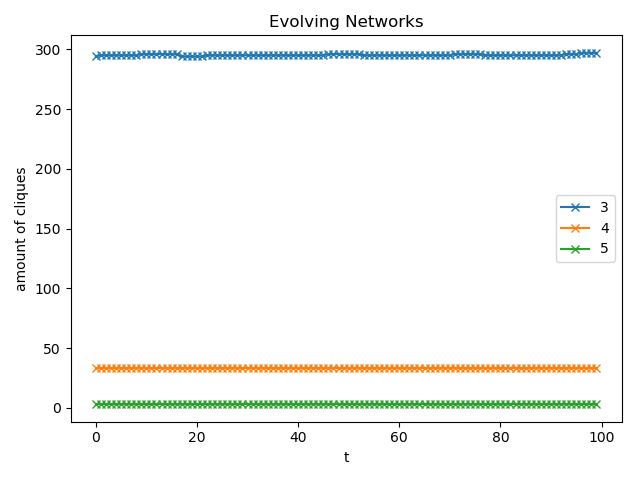
\includegraphics[scale=1]{plotTask1_100.png}
\caption{Number of cliques of size 3, 4 and 5 at the beginning and after each time step as a function of time with t = 100}
\label{fig-1}
\end{figure}

\begin{table}[!h]
\label{tab1}
\begin{tabular}{llll}
clique size & number of cliques before evolution & number of cliques after evolution\\
\hline
3 & 294 & 300\\
4 & 33 & 33\\
5 & 3 & 3\\
\end{tabular}
\caption{Number of cliques of size 3, 4 and 5 at the beginning and after letting it evolve for 100 time steps}
\end{table}

\begin{table}[!h]
\label{tab2}
\begin{tabular}{llll}
clique size & number of cliques before evolution & number of cliques after evolution\\
\hline
3 & 294 & 327\\
4 & 33 & 27\\
5 & 3 & 3\\
\end{tabular}
\caption{Number of cliques of size 3, 4 and 5 at the beginning and after letting it evolve for 1000 time steps}
\end{table}

\item The goal of randomising networks this way is to create random permutations of a network. In this way the behaviour of similar networks may be studied and the networks quality may be rated.\\
Listing \ref{ex1-2} shows source code.
\lstinputlisting[label=ex1-2,caption={Listing of source code}] {RandomizedNetwork.py}

\item Assuming a p-value of 0.05, none of the clique sizes were significantly enriched, see table \ref{tab3}.\\
Listing \ref{ex1-3} shows source code.
\lstinputlisting[label=ex1-3,caption={Listing of source code}] {MotifNetwork.py}
\begin{table}[!h]
\label{tab3}
\begin{tabular}{ll}
clique size i & $p_i$\\
\hline
3 & 0.38\\
4 & 0.27\\
5 & 1.0\\
\end{tabular}
\caption{Number of randomised networks in which the
number of cliques is at least as high as in the original network divided by the number of randomised networks for each clique size}
\end{table}
\end{enumerate}

\exercise{Annotations in Protein Protein Interaction Networks}
\begin{enumerate}
\item 

\item 

\item 

\item 

\item 
\end{enumerate}
\end{document}